\documentclass[conference]{IEEEtran}
\IEEEoverridecommandlockouts
% The preceding line is only needed to identify funding in the first footnote. If that is unneeded, please comment it out.
\usepackage{cite}
\usepackage{amsmath,amssymb,amsfonts}
%\usepackage{algorithmic}
\usepackage[]{algorithm2e} 
\usepackage{subcaption}
\usepackage{bm}
\usepackage{graphicx}
\usepackage{textcomp}
\usepackage{booktabs}
\usepackage{xcolor}

%\usepackage{xcolor}
\def\BibTeX{{\rm B\kern-.05em{\sc i\kern-.025em b}\kern-.08em
    T\kern-.1667em\lower.7ex\hbox{E}\kern-.125emX}}
\begin{document}

%\setlength\textfloatsep{5pt}  % separation of floats on bottom or top of page
%\setlength\intextsep{5pt}  % separation of floats inbetween text

\title{Inverse Analog IC Sizing and Exploration through Diffusion Models and Structural Knowledge
\thanks{%(email: filipepazevedo@gmail.com, ricmartins@lx.it.pt) (email: markus.leibl@tum.de, helmut.graeb@tum.de).\\
\textit{* Both authors contributed equally to this work.}\\
Parts of this work have been done within the collaborative project HoLoDEC funded by the Federal Ministry of Education and Research Germany (BMBF) under the funding code 16ME0705. and also funded by Fundação para a Ciência e Tecnologia – Ministério da Ciência, Tecnologia e Ensino Superior (FCT/MCTES) through national funds and, when applicable cofounded by European Union (EU) funds under the projects UIDB/50008/2020 (DOI identifier 10.54499/UIDB/50008/2020), ACTON (DOI identifier 10.54499/2023.11981.PEX), and also, by Sony Semiconductor Solutions (project GENERALISE).}}

\author{\small  Filipe $\text{Azevedo*}^{\text{1}}$, Markus $\text{Leibl*}^{\text{2}}$, Ricardo $\text{Martins}^{\text{1}}$ and Helmut $\text{Graeb}^{\text{2}}$\\ 
$^1$Instituto de Telecomunicações / Instituto Superior Técnico - Universidade de Lisboa\\
$^2$Technical University of Munich, Chair of Electronic Design Automation\\
\{filipe.p.azevedo@tecnico.ulisboa.pt, markus.leibl@tum.de, ricmartins@lx.it.pt, helmut.graeb@tum.de\}}

%\author{\IEEEauthorblockN{Markus Leibl}
%\IEEEauthorblockA{
%%\textit{Chair of Electronic Design Automation} \\
%%\textit{Technical University of Munich}\\
%%Munich, Germany \\
%markus.leibl@tum.de}
%\and
%\IEEEauthorblockN{Helmut Graeb}
%\IEEEauthorblockA{
%%\textit{Chair of Electronic Design Automation} \\
%%\textit{Technical University of Munich}\\
%%Munich, Germany \\
%helmut.graeb@tum.de}
%}


\maketitle

\begin{abstract}
In the field of analog integrated circuit sizing, the ability to rapidly and efficiently explore design spaces is crucial due to the demands of fast development cycles, evolving specifications, and increasingly complex circuits. 
It is also well established that leveraging slack in specifications through adjustments to transistor sizes can enhance yield.
To address these challenges, we propose a novel approach that combines two state-of-the-art machine learning techniques to accurately generate optimal performance points, while also enabling the exploration of nearby sizing configurations that may result in more robust designs. Specifically, we integrate a diffusion model with an algorithm that analyzes the circuit and decomposes the problem into simpler subproblems. The proposed models are evaluated on a set of typical operational amplifiers.
\end{abstract}

%\begin{IEEEkeywords}
%component, formatting, style, styling, insert
%\end{IEEEkeywords}

\section{Introduction}\label{sec:intro}
	Since the introduction of SPICE, the industry-standard method for designing analog circuits has remained largely unchanged. While the SPICE models have become increasingly complex \cite{gatermann22mosfet}, the approach of manual device tuning persists \cite{gielen23workshop}. Key challenges in making analog CAD tools useful in practice are robustness, ease of use and applicability across a high range of use cases. All those aspects are inherently difficult to grasp on a fundamental level. On the other hand, machine learning (ML) approaches excel at modeling nonlinear, black box phenomena. Their combination with already existing conventional techniques holds significant potential to bridge remaining gaps that prevent the adoption of tools in industry.
	
	Analog design is inherently an inverse problem. While the calculation of performances, yield, etc., can be reliably achieved through simulation, the reverse process - determining the optimal circuit parameters - typically relies on experience, trial and error, and complex numerical methods. As shown in previous works \cite{ leibl24inverse, lourenco19pareto}, machine learning (ML) methods can be used to accurately reproduce sizings on (Pareto) optimal fronts. Furthermore, it has been shown \cite{eid24diffusion} that diffusion models are well-suited for addressing the inverse sizing problem. Other ML-based works attempted to solve this same problem. In \cite{lourenco18}, artificial neural networks (ANNs) are used to guess circuit sizings, utilizing only one ANN for modeling an entire netlist, leading to a higher learning task complexity and thus large sample sizes are required to learn the inverse problem within a smaller performance range. In \cite{beaulieu23cascaded}, the problem is broken down into smaller tasks, and a cascade of ANNs is trained to sequentially size a single device. Each network in the cascade builds on the outputs of the previous ANNs, following a methodology similar to \cite{leibl24inverse}. The drawback is that for more complex circuits of, e.g., $15$ devices, optimally ordering the ANNs for sizing leads to a complexity of $15!\approx1.3e12$.
	
	Other works follow the traditional approach of tackling the direct sizing problem, treating it as an optimization problem \cite{fayazi23angel, budak23apostle, wolfe03nnmodel, hakhamaneshi23pretraining}. In \cite{leibl24initial} it is shown that starting points chosen via a simpler device model greatly reduce the necessary time for optimization. Reinforcement learning was also studied, with \cite{settaluri22reinforcement, zhang23multiagentRL}  replacing the optimizer with an ANN, leading to improvements in prediction speed, accuracy, and scalability. 
	However, to the best of our knowledge, none of them show strengths in all four categories, speed, accuracy, sample efficiency and exploration.
	
	In this work, we aim for a combination of all those virtues by applying denoising diffusion probabilistic models (DDPM) to the sizing of OpAmps, utilizing the approach in \cite{leibl24inverse} of subdividing the circuits into simpler structures, which has shown high accuracy for low sample sizes. DDPMs have proven their potential for generating strongly varied, but realistic results in other fields, OpenAI's DALL-E and Stable Diffusion being among the most prominent examples. As stated, \cite{eid24diffusion} proved the efficacy of these in the inverse sizing problem.
	
	Unlike most ML models, DDPMs can suggest different sizings for the same problem by repeatedly sampling them.
	As shown in Section IV, this approach to the inverse problem can produce a more varied set of sizings, which is very helpful when exploring sizing options in the vicinity of performance optima. 
This work contributes a ML approach that:
	\begin{itemize}
	\item can suggest valid sizings with resulting performance in the vicinity of the required metrics, allowing for exploration of sizings in order to pursue further optimal performance regions, while still fulfilling specifications,
	\item is highly data efficient, requiring a fraction of the dataset size used in \cite{eid24diffusion} and \cite{lourenco18},
	\item has an accurate expectation of the generated sizings,
	\item generates sizing solutions at push-button speed.
	\end{itemize}
	
 	In section \ref{sec:intro2}, we provide an overview of the proposed method and its connection to structural analysis, as well as describing the sizing process in detail. In section \ref{sec:ddpm}, a short background of DDPMs and our implemented models are presented. We conclude with a presentation of results for two OpAmps, in section \ref{sec:results}.

	 	
 	\section{From Structural Analysis to Circuit Sizing via Machine Learning}\label{sec:intro2}
	\begin{figure}[h]
		\centering
        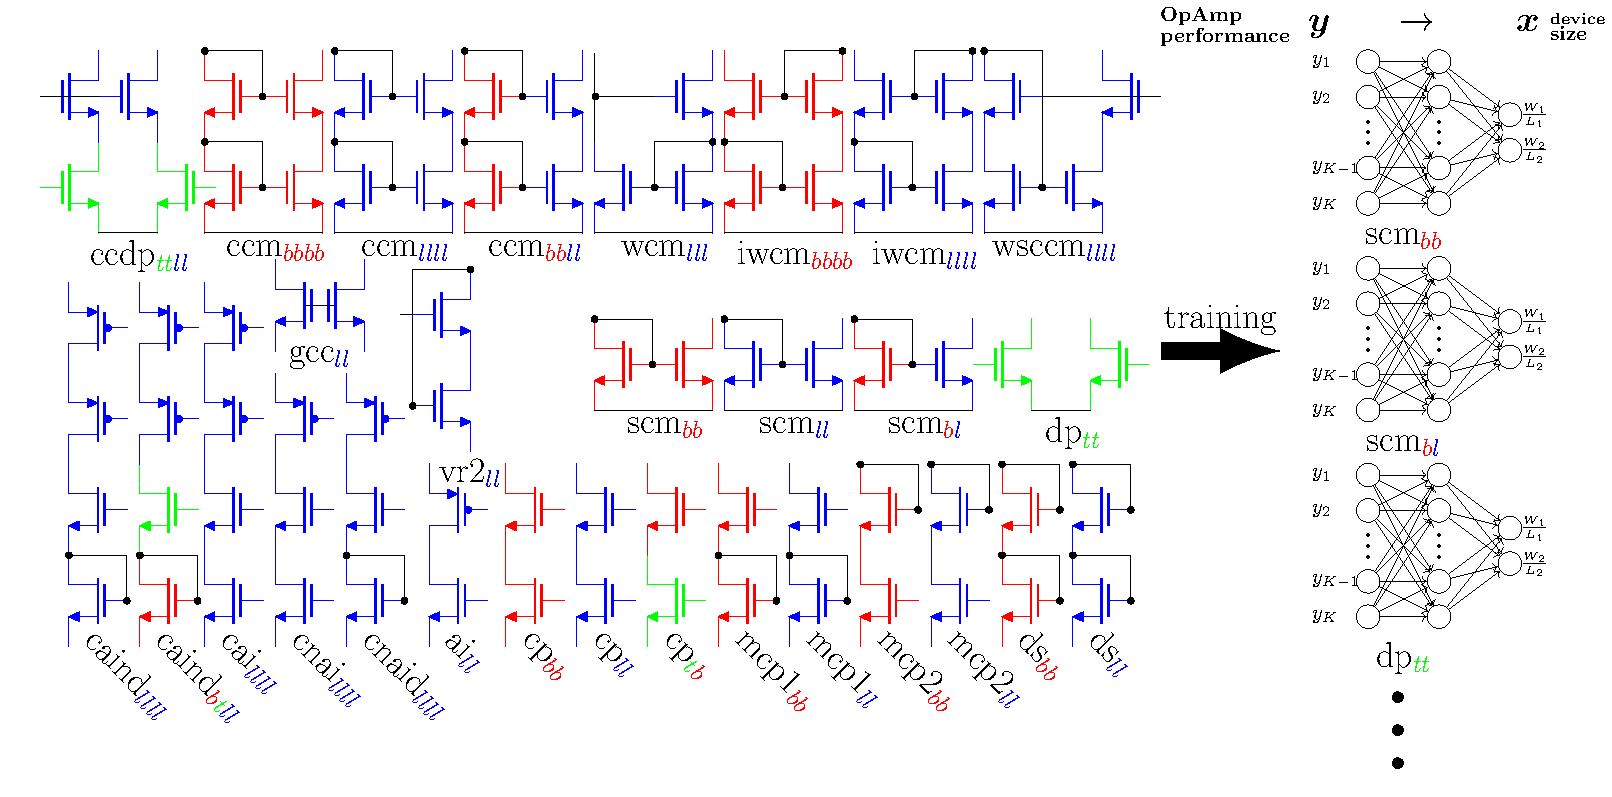
\includegraphics[width=\linewidth]{figures/struct_overview_incl_partition}
		\setlength{\abovecaptionskip}{0ex}%
		\setlength{\belowcaptionskip}{-2ex}%
		\caption{Splitting various OpAmps into canonical building blocks with different functional characteristics. Indices {\color{red} $b$}, {\color{blue} $l$} and {\color{green} $t$} represent {\color{red}$bias$}, {\color{blue}$load$} and {\color{green}$transconductance$} functionality of devices. Adapted from \cite{leibl24inverse}.}
		\label{fig:overview-structure}
	\end{figure}
	\setlength{\abovecaptionskip}{1ex}%
	\setlength{\belowcaptionskip}{-3ex}%
 	\subsection{Basics of Structural and Functional Blocks}
 	As detailed in \cite{ leibl24inverse}, the method  relies on the decomposition of circuits into subcircuits, which we call structural building blocks.
 	While the structure of the blocks is defined by their devices and interconnections, we identify three functional properties, \textit{bias, load} or \textit{transconductance}, for each individual transistor. This leads to further discrimination among the structural blocks. But because not every combination of functional properties is useful, the total set of possible structures remains small. 
	All possible variants of blocks can be found in Fig.~\ref{fig:overview-structure}.
	
	An example of decomposing a Folded-Cascode OpAmp (FCOA) into blocks can be seen in Fig.~\ref{fig:simple53}. Its structural building blocks are shaded, the names annotated close by.
	Structural and functional block recognition is fully automated. The time required for this is much less than one second. 
	
\subsection{Overview of the Method}
	\begin{figure}[]
		\centering
		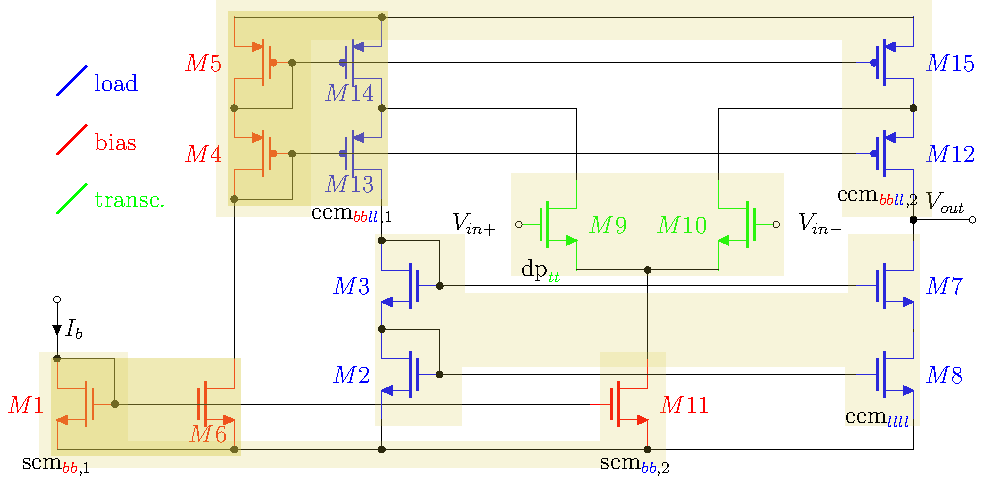
\includegraphics[width=\linewidth]{figures/simple52_partitioning}
%		\setlength{\abovecaptionskip}{0ex}%
%		\setlength{\belowcaptionskip}{-2ex}%
		\caption{Folded-Cascode OpAmp (FCOA). The circuit is decomposed into its structural and functional blocks with structural blocks shaded and functionality of the devices represented by colours. Adapted from \cite{leibl24inverse}.}
		\label{fig:simple53}
	\end{figure}
	
	In contrast to \cite{ leibl24inverse} we use a simplified version of the model. We skip the pretraining step and directly finetune the networks. Furthermore, instead of using gain boosting for sizing of $L$, we employ the same model type.
	The sizing process is then straightforward:
	\begin{itemize}
	\item split the opamp into its building blocks via \cite{abel2022fuboco}.
	\item train a neural network for each of the buidling blocks, where we use the whole OpAmp performance as guidance for the DDPM model and train to recover only the sizings of the blocks.
	\item finally, at evaluation time, recombine the predicted sizings. In case of overlap of two blocks, we take the average value.
	\end{itemize}

	Like in the previous work, we enforce symmetry that can be automatically detected by deterministic algorithms. For symmetry within blocks, this is done during training, for symmetry outside of blocks, this is done during recombination.
			

	
\section{DDPM Background and Implementation}\label{sec:ddpm}
	Several DDPMs are trained to learn the sizing and respective performance distribution of the different building blocks that make up an OpAmp. DDPMs were first introduced in \cite{ho2020denoisingdiffusionprobabilisticmodels} as a new diffusion model parametrization, which are a class of ANNs mostly used in an imaging context, like data generation and restoration. These models are composed of 3 different processes, which are briefly highlighted here:
	
	\subsubsection{Forward Process}
	First, the training data $x_{0}$ is systematically destroyed by the addition of noise over $T$ sequential steps, in the literature called timesteps, until a terminal distribution $x_{T}$ is reached. This noise is sampled from a Gaussian distribution and at the end of the $T$ timesteps, the resulting training data distribution resembles itself a Gaussian distribution. %For example, if $T=10$ then noise is sampled at each timestep and added to the data $10$ times. 
	This process is demonstrated by equation \ref{eq:forward}, where $\beta_{t}$ is the variance schedule, a hyperparameter that controls how much noise is added to the data $x$ at each time timestep $t$.
	
	\begin{equation} \label{eq:forward}
	\begin{aligned}
	q(x_{t}|x_{t-1}) &:= \mathcal{N}(x_{t};\mu,\Sigma) \\ &:= \mathcal{N}(x_{t};\sqrt{1-\beta_{t}}x_{t-1}, \beta_{t}I)
	\end{aligned}
	\end{equation}
	
	\subsubsection{Reverse Process}
	After the data is destroyed until $x_{t}$, an ANN is trained to try to reverse the forward process, either by predicting the original data $x_{0}$ up front, or by predicting another value that can be used to reconstruct the original data, like the added noise $\epsilon$, etc. This process is represented by equation \ref{eq:reverse}, where $\alpha_{t}=1-\beta_{t}$ and $\overline{\alpha}_{t}=\prod_{s=1}^{t}\alpha_{s}$.
	
	\begin{equation} \label{eq:reverse}
	\begin{split}
		\rho_{\theta}(x_{t-1}|x_{t}) := \mathcal{N}(x_{t-1};\mu_{\theta}(x_{t},t),\Sigma_{\theta}(x_{t},t)) \\:= \mathcal{N}(x_{t};\frac{1}{\sqrt{\alpha_{t}}}(x_{t}-\frac{1-\alpha_{t}}{\sqrt{1-\overline{\alpha}_{t}}}\epsilon_{\theta}(x_{t},t)),\beta_{t}I) 
	\end{split}
	\end{equation}
	
	The correlation between the forward and reverse process to noise and denoise images can be seen in Fig.~\ref{fig:forward_reverse}. An overview of the training phase for the FCOA of Fig.~\ref{fig:simple53} can be seen in Fig.~\ref{fig:DDPMtraining}.
	
	\begin{figure}[h]
		\centering
		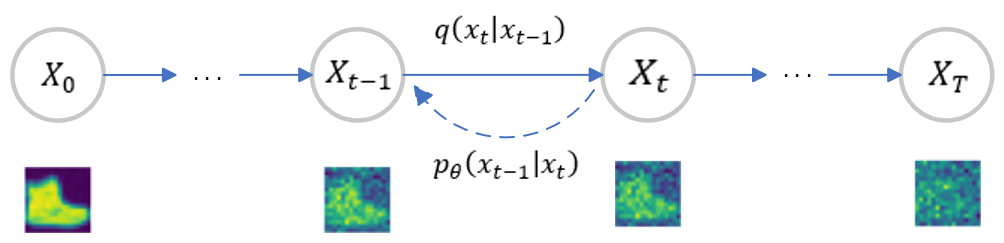
\includegraphics[width=\linewidth]{figures/ForwardReverseDDPM}
		\setlength{\abovecaptionskip}{0ex}%
		\setlength{\belowcaptionskip}{-2ex}%
		\caption{Correlation between forward and reverse processes \cite{eid24diffusion}.}
		\label{fig:forward_reverse}
	\end{figure}
	
	\begin{figure}[h]
		\centering
		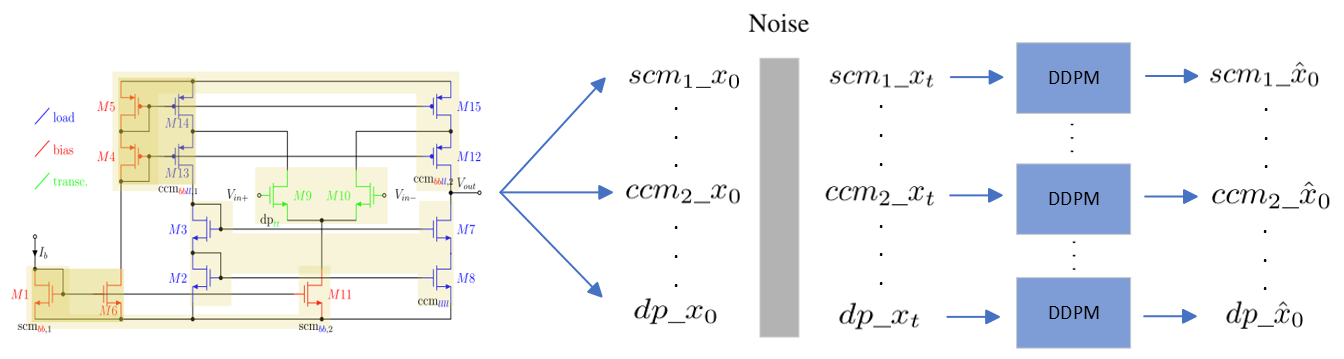
\includegraphics[width=\linewidth]{figures/DDPMSubBlockTraining}
		\setlength{\abovecaptionskip}{0ex}%
		\setlength{\belowcaptionskip}{-2ex}%
		\caption{Training phase for sizing an OpAmp. After the decomposition into sub-blocks, noise is added to the respective sizings. A DDPM is trained for each sub-block to predict the original sizing values. The respective performances of the original sizings are given as guidance.}
		\label{fig:DDPMtraining}
	\end{figure}
	
	\subsubsection{Sampling Process}
	Finally, after the model is trained, the sampling process is used to generate new data. The model learned to reverse the forward process, and so, when giving it pure Gaussian noise, it tries to reverse the noise addition until arriving at the original data. Except this time, there is no actual data to begin with, marking this a form of generative artificial intelligence. This stage is similar to the training phase shown in Fig. \ref{fig:DDPMtraining}, except random noise is given as input to the network instead of the noisy sizings.
	
	It was shown by \cite{eid24diffusion} that DDPMs produce interesting results when applied to the inverse sizing problem. In this work, a similar implementation is considered, with a cosine schedule without clipping \cite{lin2024commondiffusionnoiseschedules} for $\beta_t$ and classifier-free guidance \cite{ho2022classifierfreediffusionguidance}, but with 2 key differences:
	
	\begin{itemize}
		\item instead of predicting the noise $\epsilon$, we implement a model that predicts a velocity equation $v_{t}=\alpha_{t}\epsilon - \sigma_{t}x$ which has been shown to enable a true signal-to-noise ratio of $0$ at the last timestep $T$ (meaning that at the last timstep the input of the model is pure Gaussian noise), as opposed to other DDPM parametrizations. This removes an important discrepancy between training (where the model would never see pure noise) and inference \cite{lin2024commondiffusionnoiseschedules};
		\item the backbone of the model implemented  is a transformer, with an architecture similar to the ``adaLN-Zero'' model of  \cite{peebles2023scalablediffusionmodelstransformers}, as opposed to the simple multi-layer perceptrons implemented by \cite{eid24diffusion}. To predict a more complex value in $v$, a stronger architecture was required.
	\end{itemize}
	
	
	
	\section{Experimental Results} \label{sec:results}
	\begin{figure}[]
		\centering
		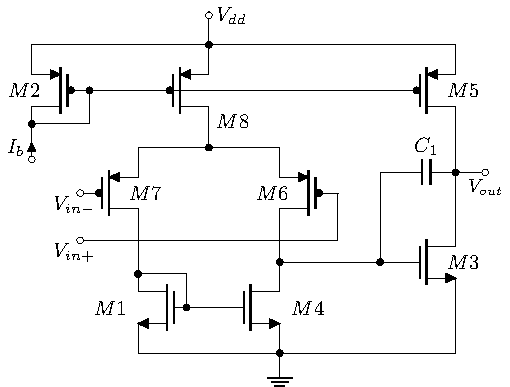
\includegraphics[width=.5\linewidth]{figures/miller_pmos}
		%		\setlength{\abovecaptionskip}{0ex}%
		%		\setlength{\belowcaptionskip}{-2ex}%
		\caption{Miller OpAmp (MOA)}
		\label{fig:miller}
	\end{figure}
	
	\begin{figure}[]
		\begin{subfigure}{.5\textwidth}
			\centering
			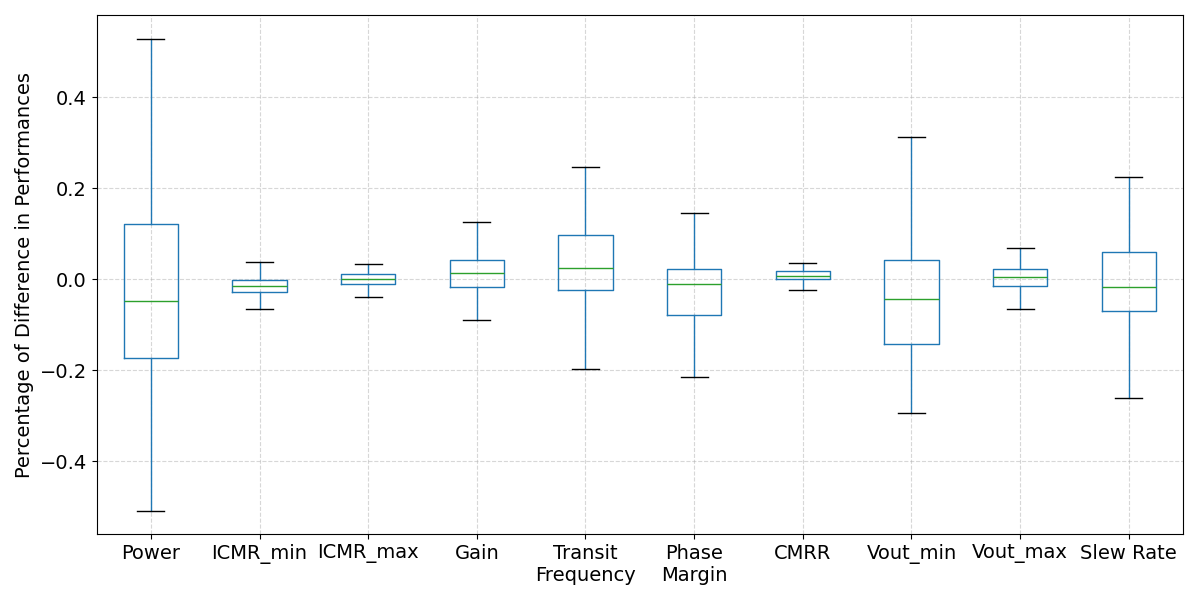
\includegraphics[width=\linewidth]{figures/BoxplotFCA}
			\setlength{\abovecaptionskip}{0ex}%
			%		\setlength{\belowcaptionskip}{-2ex}%
			\setlength{\belowcaptionskip}{0ex}%
			\caption{FCOA.}
			\label{fig:boxplotfca}
		\end{subfigure}
		\hfill
		\begin{subfigure}{.5\textwidth}
			\centering
			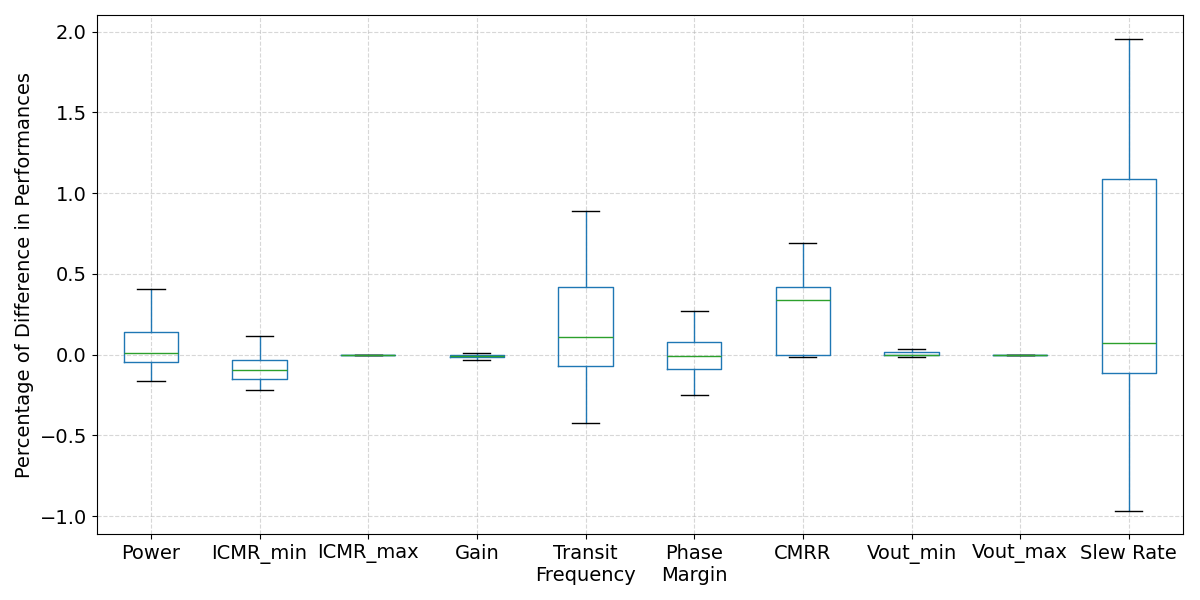
\includegraphics[width=\linewidth]{figures/BoxplotMillerOpAmp}
			\setlength{\abovecaptionskip}{-0.5ex}%
			%		\setlength{\belowcaptionskip}{-2ex}%
			\caption{MOA.}
			\label{fig:boxplotmiller}
		\end{subfigure}
		\setlength{\abovecaptionskip}{3ex}%
		\setlength{\belowcaptionskip}{-4ex}%
		%			\caption{Folded Cascode OpAmp (\ref{fig:simple53}) and process of transfer learning (\ref{fig:fine-tuning}): Instead of training one huge network per OpAmp, we can use weights from our database as initial training points to merely fine-tune our networks }
		\caption{Boxplots of the percentage of differences in performances for the test set of both tested OpAmps, after removal of outliers. The innermost line represents the median, the box $50\%$ of the data. }
		\label{fig:boxplots}
	\end{figure}
	

	We trained our approach on two different OpAmps, the FCOA previously studied in \cite{leibl24inverse} shown in Fig. \ref{fig:simple53} and the Miller OpAmp (MOA) in Fig. \ref{fig:miller}. %After training, we sampled the models for all ground truth sizings in the test sets of both OpAmps, corresponding to 118 for the FCOA and 77 for the Miller OpAmp. 
	After training, we sampled the models for all elements in the test sets (containing specification and a ground truth sizing) of both OpAmps, corresponding to $118$ for the FCOA and $77$ for the Miller OpAmp. 
	After simulating the sampled values, the resulting performances were compared with simulations of the ground truth values. 
	All models have been trained with a sample size between $700$ and $1000$ elements. While slightly less efficient than \cite{leibl24inverse}, the price for added flexibility, the sample sizes are still very low.
	
	Boxplots of the relative performance differences are presented in Fig.~\ref{fig:boxplots}, bar outliers.
	For the FCOA in Fig.~\ref{fig:boxplotfca}, most boxes are centered around $0$ (i.e. the ground truth), but some performances show a tendency of improvement. For Power, ICMR\textsubscript{min} and Vout\textsubscript{min} median and box extend downwards (the predictions' performances are lower than the labels), while Gain and Transit Frequency median and box extend upwards (the predictions' performances are greater than the ground truth sizings). Similar observations can be made for the MOA in Fig.~\ref{fig:boxplotmiller}, with the CMRR and Slew Rate having the biggest improvement. Here, the only performance that showed a tendency toward deterioration was Power. This shows that the models are able to accurately learn the distribution of the circuits' sizing and respective performances, sometimes finding interesting improvements that might be attributed to learned trade-offs between sizes of the different sub-blocks.
	
	In a second experiment we sampled the model for the FCOA $100$ times, while keeping the same performance specification. The results can be seen in Fig.~\ref{fig:histograms53} and Table~\ref{tab:device_stats}. Most distributions in the performance space in Fig.~\ref{fig:histograms53} exhibit a gaussian behaviour, centered around the ground truth performance marked by a red star. Table~\ref{tab:device_stats} indicates that the model learns to estimate the different contributions and sensitivities for the individual parameters. It can be seen that the standard deviation varies heavily depending on the device, indicating that the model learns to scale the effects of parameter deviations.

	\setlength{\textfloatsep}{0.4cm}
	\begin{table}[]
%		\tiny
		\centering
		\setlength{\abovecaptionskip}{0ex}%
		\setlength{\belowcaptionskip}{2ex}%
		\caption{Estimated mean value and standard deviation of W parameter sizes of the FCOA for 100 samples and same performance specification.}
		\label{tab:device_stats}
		\resizebox{.6\linewidth}{!}{
		\begin{tabular}{lll}
		\toprule
	 device & mean value $[\mu m]$ & standard deviation \\ 
	 \midrule
		0 & $8.52$ & $2.0$ \\
		1 & $43.26$ & $19.0$ \\
		2 & $41.74$ & $17.0$ \\
		3 & $14.4$ & $1.0$ \\
		4 & $90.98$ & $8.0$ \\
		5 & $88.47$ & $23.0$ \\
		6 & $41.74$ & $17.0$ \\
		7 & $43.26$ & $19.0$ \\
		8 & $97.88$ & $55.0$ \\
		9 & $97.88$ & $55.0$ \\
		10 & $114.78$ & $35.0$ \\
		11 & $367.21$ & $22.0$ \\
		12 & $367.21$ & $22.0$ \\
		13 & $244.11$ & $13.0$ \\
		14 & $244.11$ & $13.0$ \\
		\bottomrule
		\end{tabular}
		\vspace{-5cm}
		
		}\end{table}
		
%	\setlength{\textfloatsep}{0.6cm}
	\begin{figure}[]
		\centering
		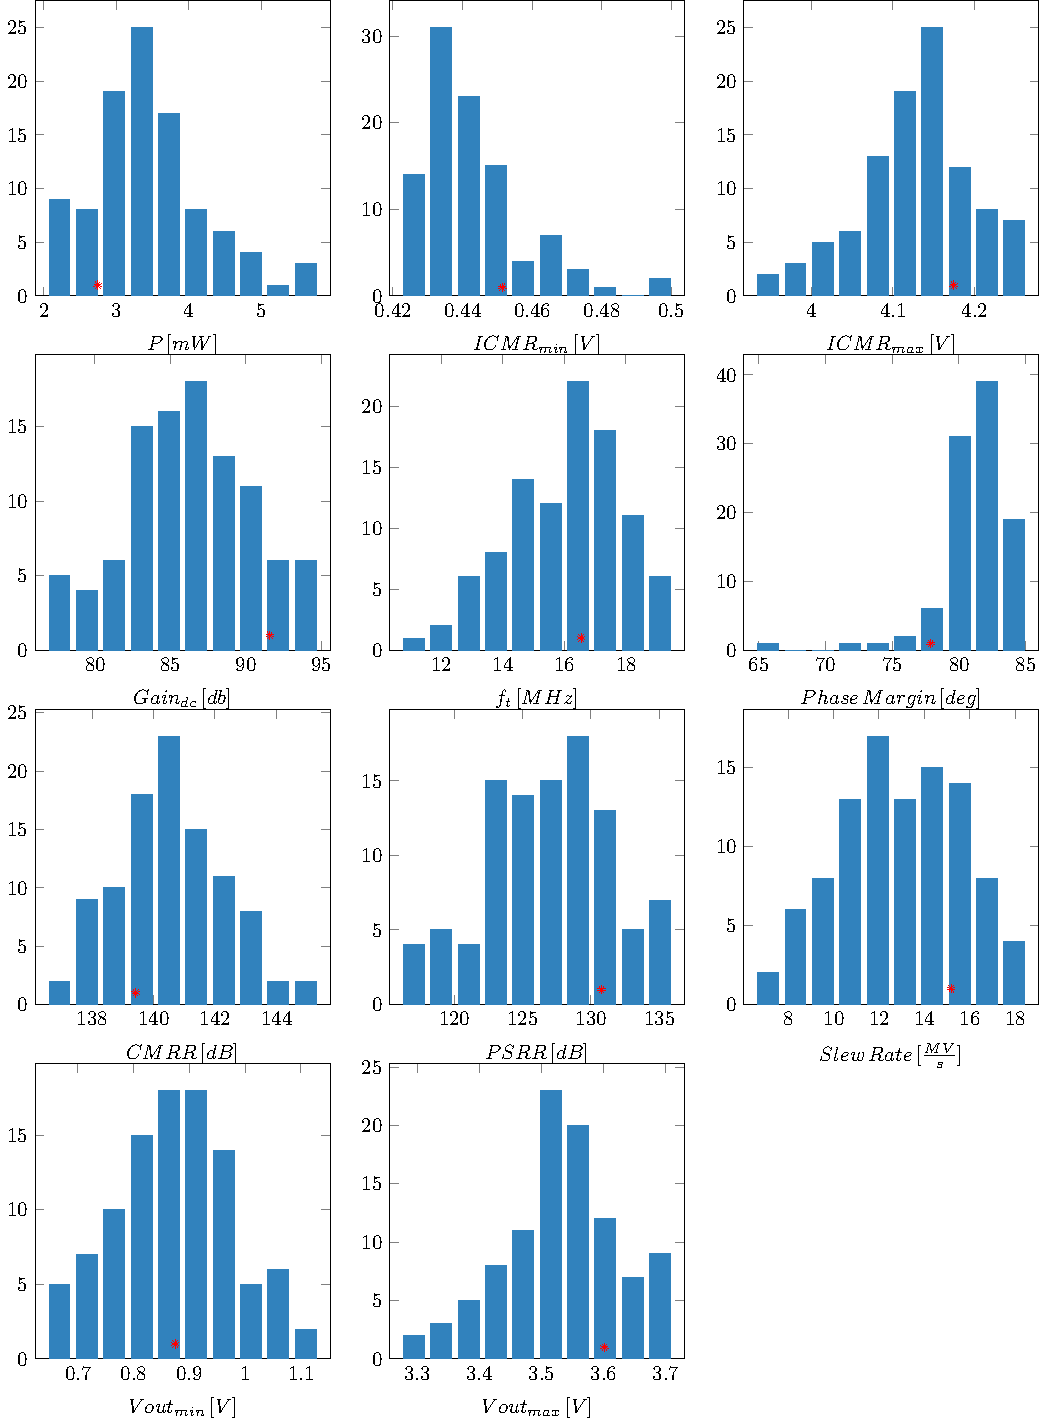
\includegraphics[width=\linewidth]{figures/histograms_simple53_100samples}
%		\setlength{\abovecaptionskip}{0ex}%
%		\setlength{\belowcaptionskip}{-2ex}%
		\caption{Histograms for $100$ samples of the trained FCOA model with \textbf{same} performance specification. Most distributions are well shaped around the ground truth from the test set. A red star marks the performance value of the ground truth sizing.}
		\label{fig:histograms53}
	\end{figure}
	
	
\section{Conclusion}
	We have shown a machine learning approach to not only reproduce optimal sizings for a given specification, but also to help explore points in the nearby performance space. In the scenario of sampling multiple times for the same specification, the sampling can be interpreted as adding random noise to the ground truth sizing. The model learns the corresponding covariance matrix. As the standard deviation is not equal for all devices, this behaviour cannot be mimicked by simply adding noise to an optimal sizing.

\bibliographystyle{IEEEtran}
\bibliography{IEEEabrv,bibtex-base-iee}

\end{document}
